\section{Cronograma}

O processo de desenvolvimento será separado em 3 tópicos principais, inteligência artificial, diagrama de Voronoi e interface de usuário. O desenvolvimento de cada tópico do software será feito em paralelo, pois os tópicos não possuem acoplamento.

\subsection*{inteligência Artificial}

Será necessário decidir quais conjuntos de dados utilizar, o modelo está pronto e disponível no GitHb \cite{mohan2020efficientps} portanto será necessário treinar o modelo e avalia-lo com base na métrica PQ \cref{eq:pg_metric}.

As especificações do modelo proposto são: Linux, Python 3.7, PyTorch 1.7, CUDA 10.2, GCC 7 ou 8 além dos pacotes inseridos no arquivo requirements.txt.

O tempo estimado para o desenvolvimento é de 1 a 2 meses, a maior parte será para treinar e validar o resultado.

\subsection*{Diagrama de Voronoi}

Para o desenvolver código do diagrama de Voronoi será preciso primeiro gerar os pontos e desses pontos as áreas, fazer o algoritmo entender se a área tocou no segmento de imagem, caso tenha tocado armazenar para um processamento posterior que irá especificar qual bioma aquela áreas será, para fazer os teste será necessário uma imagem com um polígono.

O tempo estimado para o desenvolvimento é de 1 mes.

\subsection*{Interface de Usuário}

A interface de usuárioterá5 telas principais, início, processamento da segmentação, seleção, processamento de seleção, resultado. 

As telas terão o seguinte fluxo:

\begin{figure}[H]
	\centering
    \caption{Tela de início, botões de carregar imagem e carregar projeto, menu de contexto arquivos com 3 botões, carregar imagem, carregar projeto e salvar.}
	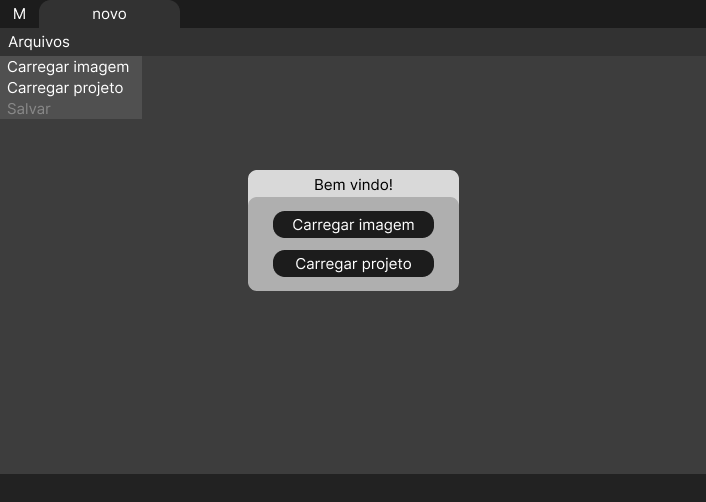
\includegraphics[width=0.55\textwidth]{figures/tela_novo.png}
    \legend{Fonte: Criação própria}
	\label{fig:tela_novo}
\end{figure}


\begin{figure}[H]
	\centering
    \caption{Tela de processamento da segmentação}
	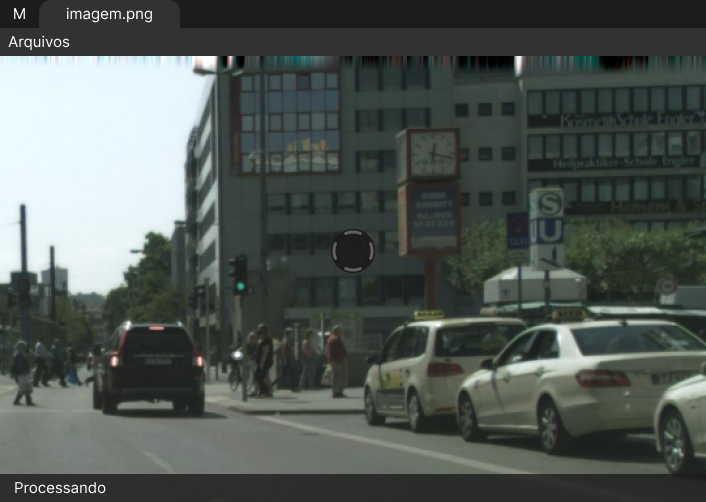
\includegraphics[width=0.55\textwidth]{figures/tela_processando_1.png}
    \legend{Fonte: Criação própria}
	\label{fig:tela_processando_1}
\end{figure}


\begin{figure}[H]
	\centering
    \caption{Tela de seleção de segmentação da imagem.}
	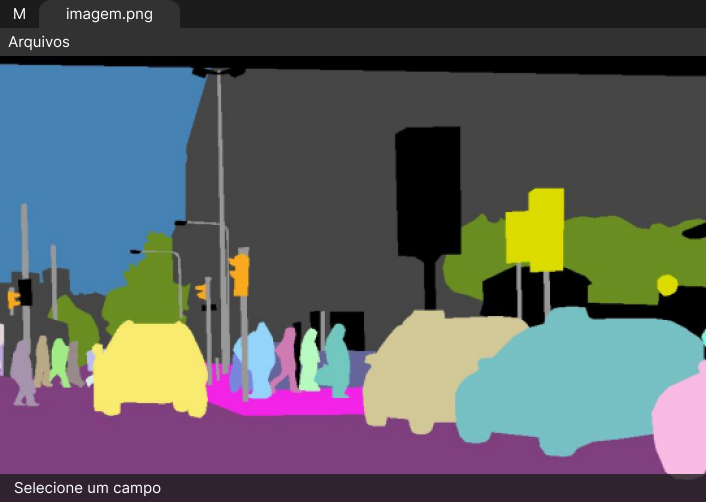
\includegraphics[width=0.8\textwidth]{figures/tela_carregado.png}
    \legend{Fonte: Criação própria}
	\label{fig:tela_carregado}
\end{figure}


\begin{figure}[H]
	\centering
    \caption{Tela de processamento para geração do mapa com a seleção do segmento.}
	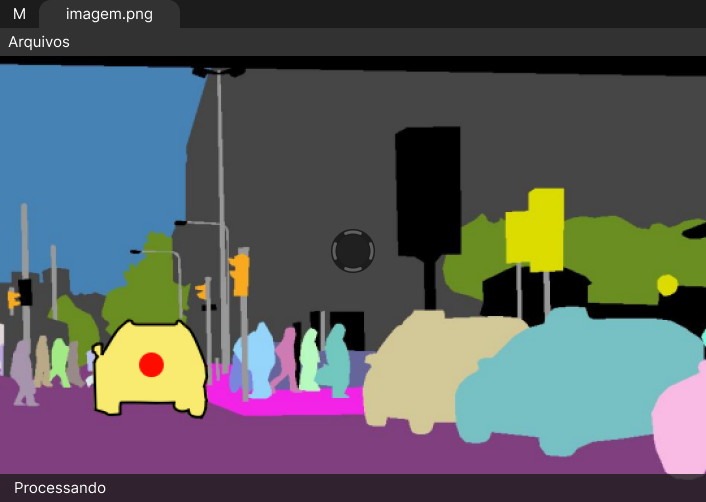
\includegraphics[width=0.8\textwidth]{figures/tela_processando_2.png}
    \legend{Fonte: Criação própria}
	\label{fig:tela_processando_2}
\end{figure}


\begin{figure}[H]
	\centering
    \caption{Tela de resultado com o mapa gerado após processamento.}
	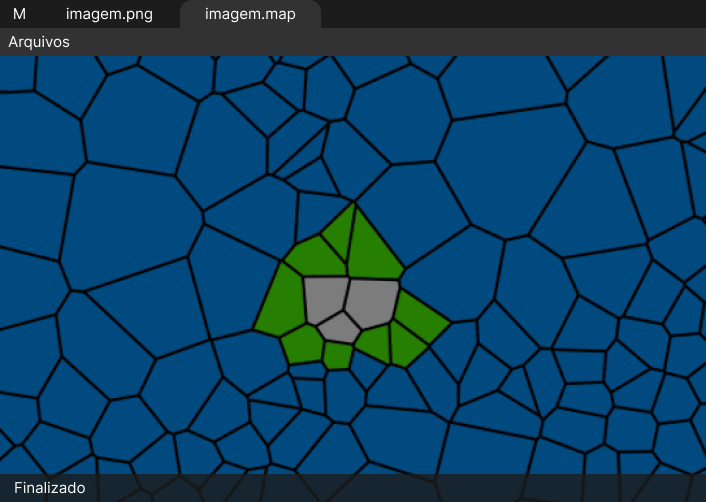
\includegraphics[width=0.6\textwidth]{figures/tela_mapa.png}
    \legend{Fonte: Criação própria}
	\label{fig:tela_mapa}
\end{figure}

Após isso a interface permitirá o usuário salvar o projeto bem como exportar o resultado.

O tempo de desenvolvimento será em torno de 1 mês.
